\section{Detailed view of the approach}
\label{sec:S1}

Figure~\ref{fig:demarche-detail} details the approach summarized in Figure~1 of the main manuscript. For each of the three blocks, it specifies the inputs, the processing steps, and the outputs: the generation of labeled crises and their four versions (Simulate), the fitting of the resilience curve and the computation of the indicators (Measure), and the learning of the causal Bayesian network and its three uses (Learn). Thumbnails show a trajectory, a fitted curve, and the structure of the learned network.

\begin{center}\begin{minipage}{\textwidth}\centering
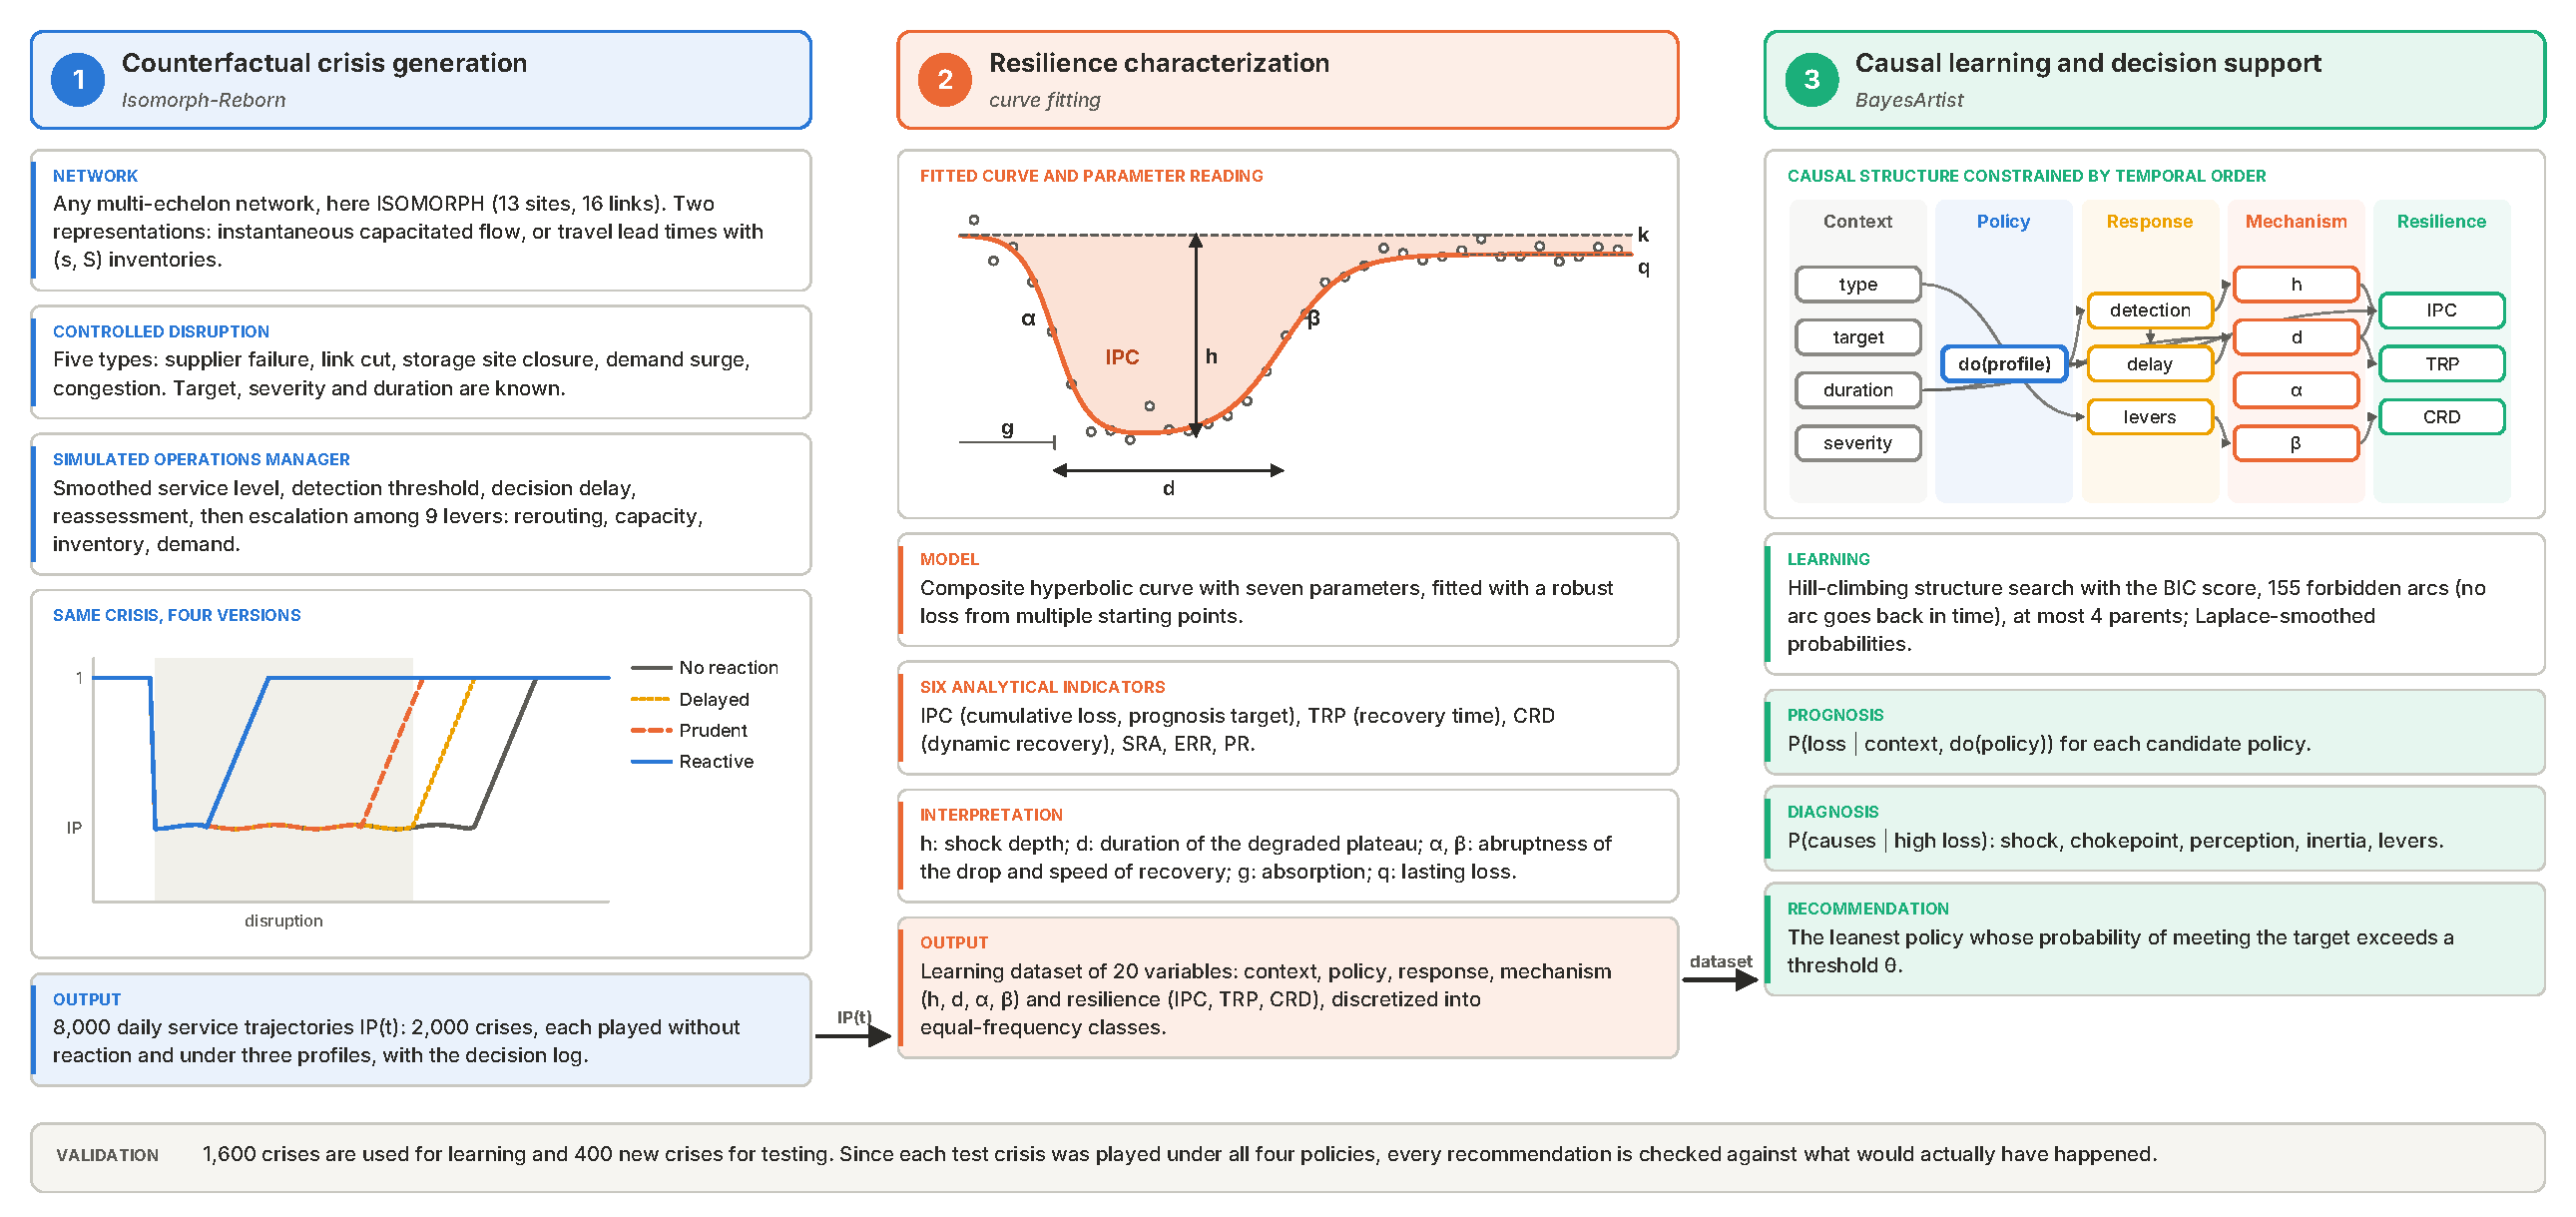
\includegraphics[width=\textwidth]{figures/Fig1_approach_EN.pdf}
\captionof{figure}{Detailed three-block approach: inputs, processing steps, and outputs of each block.}\label{fig:demarche-detail}
\end{minipage}\end{center}
